\documentclass[border=6pt]{standalone}
\usepackage{fontspec}
\usepackage[sfdefault,lining]{FiraSans}
\usepackage{pgfplots}
\usepgfplotslibrary{groupplots}
\pgfplotsset{compat=1.18}
\definecolor{tsnavy}{HTML}{1A2E4F}\definecolor{tsred}{HTML}{A6252D}\definecolor{tsink}{HTML}{1F2430}
\definecolor{tsgrey}{HTML}{5F6B7C}\definecolor{tsmuted}{HTML}{A7B2C2}\definecolor{tsline}{HTML}{D6DCE5}
\definecolor{cRepair}{HTML}{1B7F9E}\definecolor{cControl}{HTML}{C98A2B}
\definecolor{cVanOurs}{HTML}{F2C3C6}\definecolor{cVanPaper}{HTML}{8AA4CC}
\pgfplotsset{rd/.style={axis lines*=left, ymajorgrids, grid style={tsline,line width=0.4pt},
  axis line style={tsgrey,line width=0.5pt}, major tick style={draw=none},
  tick label style={font=\small,text=tsgrey,/pgf/number format/assume math mode=true}, label style={font=\small,text=tsink},
  title style={font=\bfseries\color{tsnavy}},
  legend style={draw=none,fill=none,font=\small,text=tsink,/tikz/every even column/.append style={column sep=10pt}},
  legend cell align=left, every axis plot/.append style={line width=0.5pt}}}
\begin{document}
\pagecolor{white}
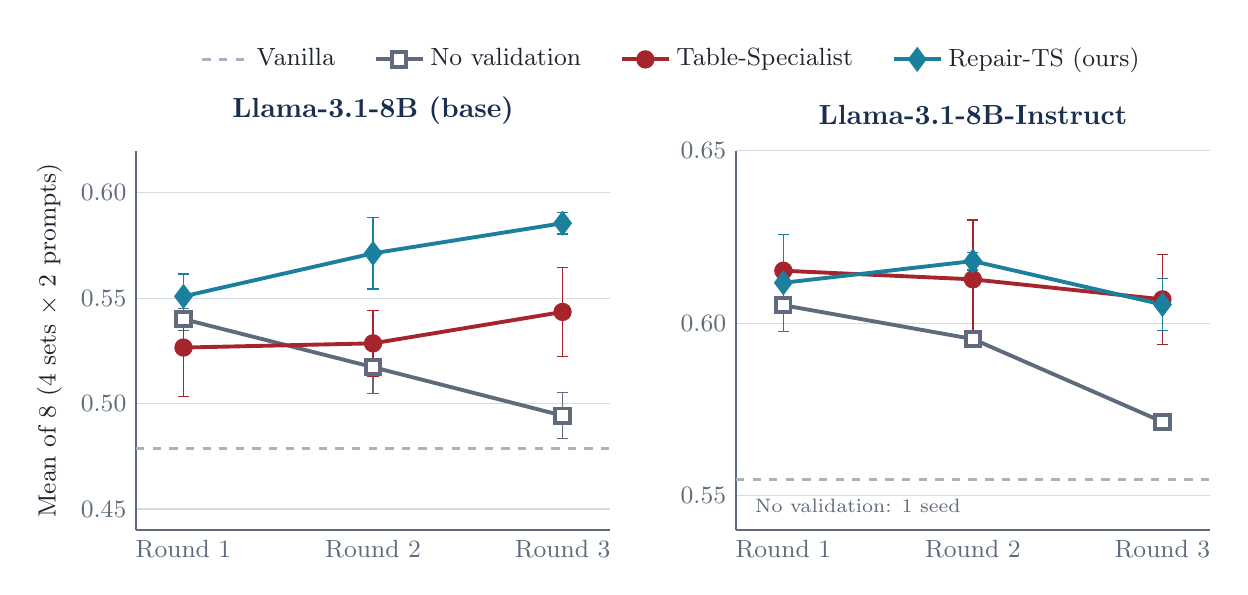
\begin{tikzpicture}
\begin{groupplot}[group style={group size=2 by 1, horizontal sep=1.6cm}, rd, width=7.6cm, height=6.4cm,
  xmin=0.75, xmax=3.25, xtick={1,2,3}, y tick label style={/pgf/number format/.cd,fixed,fixed zerofill,precision=2}, xticklabels={Round 1,Round 2,Round 3},
  error bars/error bar style={line width=0.6pt}, error bars/error mark options={rotate=90,mark size=2pt},
  every axis plot/.append style={line width=1.4pt, mark size=2.6pt}]
\nextgroupplot[title={Llama-3.1-8B (base)}, ymin=0.44, ymax=0.62, ylabel={Mean of 8 (4 sets $\times$ 2 prompts)},legend to name=roundslegend, legend columns=4,legend style={draw=none,font=\small,/tikz/every even column/.append style={column sep=12pt}}]
\addplot[tsmuted,dashed,mark=none,line width=1.1pt,domain=0.75:3.25] {0.4788};
\addplot[tsgrey,mark=square*,mark options={fill=white},error bars/.cd,y dir=both,y explicit] coordinates {(1,0.5401) +- (0,0.0052) (2,0.5173) +- (0,0.0123) (3,0.4943) +- (0,0.0108)};
\addplot[tsred,mark=*,error bars/.cd,y dir=both,y explicit] coordinates {(1,0.5266) +- (0,0.0232) (2,0.5286) +- (0,0.0155) (3,0.5435) +- (0,0.0210)};
\addplot[cRepair,mark=diamond*,mark size=3.4pt,error bars/.cd,y dir=both,y explicit] coordinates {(1,0.5509) +- (0,0.0106) (2,0.5713) +- (0,0.0169) (3,0.5856) +- (0,0.0051)};
\legend{Vanilla,No validation,Table-Specialist,Repair-TS (ours)}
\nextgroupplot[title={Llama-3.1-8B-Instruct}, ymin=0.54, ymax=0.65, ylabel={}]
\addplot[tsmuted,dashed,mark=none,line width=1.1pt,domain=0.75:3.25] {0.5546};
\addplot[tsgrey,mark=square*,mark options={fill=white},error bars/.cd,y dir=both,y explicit] coordinates {(1,0.6052) +- (0,0.0000) (2,0.5954) +- (0,0.0000) (3,0.5714) +- (0,0.0000)};
\addplot[tsred,mark=*,error bars/.cd,y dir=both,y explicit] coordinates {(1,0.6152) +- (0,0.0106) (2,0.6127) +- (0,0.0172) (3,0.6069) +- (0,0.0131)};
\addplot[cRepair,mark=diamond*,mark size=3.4pt,error bars/.cd,y dir=both,y explicit] coordinates {(1,0.6117) +- (0,0.0140) (2,0.6180) +- (0,0.0026) (3,0.6054) +- (0,0.0075)};
\node[font=\scriptsize,text=tsgrey,anchor=south west] at (rel axis cs:0.02,0.02) {No validation: 1 seed};
\end{groupplot}
\node[anchor=south] at ($(group c1r1.north)!0.5!(group c2r1.north)+(0,0.75cm)$) {\pgfplotslegendfromname{roundslegend}};
\end{tikzpicture}
\end{document}
